\documentclass[serif]{beamer}\usepackage[]{graphicx}\usepackage[]{color}
%% maxwidth is the original width if it is less than linewidth
%% otherwise use linewidth (to make sure the graphics do not exceed the margin)
\makeatletter
\def\maxwidth{ %
  \ifdim\Gin@nat@width>\linewidth
    \linewidth
  \else
    \Gin@nat@width
  \fi
}
\makeatother

\definecolor{fgcolor}{rgb}{0.345, 0.345, 0.345}
\newcommand{\hlnum}[1]{\textcolor[rgb]{0.686,0.059,0.569}{#1}}%
\newcommand{\hlstr}[1]{\textcolor[rgb]{0.192,0.494,0.8}{#1}}%
\newcommand{\hlcom}[1]{\textcolor[rgb]{0.678,0.584,0.686}{\textit{#1}}}%
\newcommand{\hlopt}[1]{\textcolor[rgb]{0,0,0}{#1}}%
\newcommand{\hlstd}[1]{\textcolor[rgb]{0.345,0.345,0.345}{#1}}%
\newcommand{\hlkwa}[1]{\textcolor[rgb]{0.161,0.373,0.58}{\textbf{#1}}}%
\newcommand{\hlkwb}[1]{\textcolor[rgb]{0.69,0.353,0.396}{#1}}%
\newcommand{\hlkwc}[1]{\textcolor[rgb]{0.333,0.667,0.333}{#1}}%
\newcommand{\hlkwd}[1]{\textcolor[rgb]{0.737,0.353,0.396}{\textbf{#1}}}%

\usepackage{framed}
\makeatletter
\newenvironment{kframe}{%
 \def\at@end@of@kframe{}%
 \ifinner\ifhmode%
  \def\at@end@of@kframe{\end{minipage}}%
  \begin{minipage}{\columnwidth}%
 \fi\fi%
 \def\FrameCommand##1{\hskip\@totalleftmargin \hskip-\fboxsep
 \colorbox{shadecolor}{##1}\hskip-\fboxsep
     % There is no \\@totalrightmargin, so:
     \hskip-\linewidth \hskip-\@totalleftmargin \hskip\columnwidth}%
 \MakeFramed {\advance\hsize-\width
   \@totalleftmargin\z@ \linewidth\hsize
   \@setminipage}}%
 {\par\unskip\endMakeFramed%
 \at@end@of@kframe}
\makeatother

\definecolor{shadecolor}{rgb}{.97, .97, .97}
\definecolor{messagecolor}{rgb}{0, 0, 0}
\definecolor{warningcolor}{rgb}{1, 0, 1}
\definecolor{errorcolor}{rgb}{1, 0, 0}
\newenvironment{knitrout}{}{} % an empty environment to be redefined in TeX

\usepackage{alltt}
\usetheme{Boadilla}
\usetheme{Boadilla}
\usepackage{graphicx}
\usepackage[final]{animate}
\usepackage{breqn}
\usepackage{xcolor}
\usepackage{booktabs}
\usepackage{tikz}
\usetikzlibrary{decorations.pathreplacing}
\usetikzlibrary{shapes,arrows,positioning,shadows}
\definecolor{links}{HTML}{2A1B81}
\hypersetup{colorlinks,linkcolor=links,urlcolor=links}
\usepackage{subfig}
\usepackage{pgf}

% load R libraries


% custom colors, do not cache
\definecolor{mypal1}{HTML}{F0F9E8}\definecolor{mypal2}{HTML}{BAE4BC}\definecolor{mypal3}{HTML}{7BCCC4}\definecolor{mypal4}{HTML}{43A2CA}\definecolor{mypal5}{HTML}{0868AC}

% my custom ggplot theme

 
% knitr and global options


% colors and macros
\setbeamercolor{title}{fg=mypal5} % main title
\setbeamercolor{frametitle}{fg=mypal4, bg=mypal2} % frame titles
\setbeamercolor{structure}{fg=mypal4} % bottom banner
\setbeamercolor{normal text}{fg=mypal5}
\usebackgroundtemplate{
\includegraphics[height=\paperheight,width=\paperwidth]{fig/back_tmp.pdf}}

\tikzstyle{block} = [rectangle, draw, text width=9em, text centered, rounded corners, minimum height=3em, minimum width=7em, top color = white, bottom color=brown!30,  drop shadow]

\newcommand{\ShowSexpr}[1]{\texttt{{\char`\\}Sexpr\{#1\}}}

\newcommand{\Bigtxt}[1]{\textbf{\textit{#1}}}
\IfFileExists{upquote.sty}{\usepackage{upquote}}{}
\begin{document}

\titlegraphic{
\centerline{
\fbox{
\includegraphics[width=0.7\textwidth]{fig/swmprats_logo.png}}}
}

\title[NERRS Analysis Tools]{Integrated Analysis Tools for the NERRS System-Wide Monitoring Program Data}

\author[M. Beck, T. O'Brien, M. Bundy]{Marcus W. Beck\inst{1} \and Todd D. O'Brien\inst{2} \and Marie H. Bundy\inst{2}}

\date{May 5, 2016}

\institute[]{\inst{1} USEPA NHEERL Gulf Ecology Division\\ Email: \href{mailto:beck.marcus@epa.gov}{beck.marcus@epa.gov} \and \inst{2} NERRS/NMFS/NOAA \\ Emails: \href{mailto:todd.obrien@noaa.gov}{todd.obrien@noaa.gov}, \href{mailto:marie.bundy@noaa.gov}{marie.bundy@noaa.gov}}

%%%%%%
\begin{frame}
\vspace{-0.1in}
\titlepage
\end{frame}

%%%%%%
\begin{frame}{
\includegraphics[width=0.05\paperwidth]{fig/muskrat.png}\hspace{0.07in}{\bf Overview}}
\begin{itemize}
\item Background of National Estuarine Research Reserves (NERRS) System-wide Monitoring Program (SWMP) \\~\\
\item Genesis of ``SWMPrats.net'' community of practice \\~\\
\item Features of SWMPrats.net \\~\\
\begin{itemize}
\item SWMPr \\~\\
\item widgets \\~\\
\item forum \\~\\
\end{itemize}
\item Continuing work, training, and engagement
\end{itemize}
\end{frame}

%%%%%%
\begin{frame}{What is NERRS/SWMP?}{}
{\bf NERRS}\\
National Estuarine Research Reserve System, established by Coastal Zone Management Act of 1972. Focus on \Bigtxt{long-term research}, \Bigtxt{monitoring}, \Bigtxt{education}, and \Bigtxt{stewardship} for more effective coastal management.\\~\\
{\bf SWMP}\\
System Wide Monitoring Program, initiated in 1995 to provide \Bigtxt{continuous monitoring} data at over 300 stations in in each of the 28 NERRS reserves \\~\\
\end{frame}

%%%%%%
\begin{frame}{What is NERRS/SWMP?}
\centerline{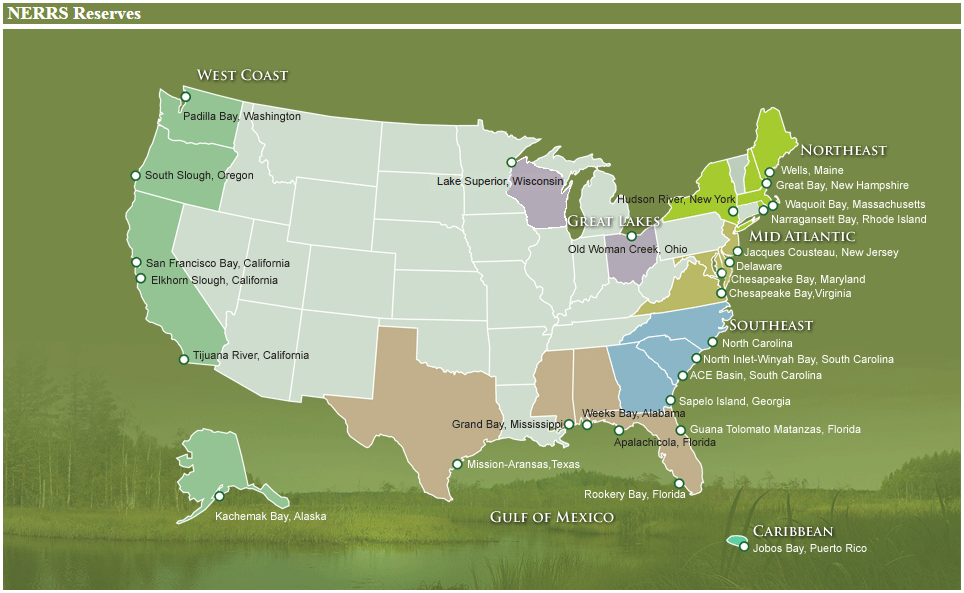
\includegraphics[width = 0.9\textwidth]{fig/NERRS_locations.png}}
\tiny
\flushright
\href{http://nerrs.noaa.gov/ReservesMap.aspx}{http://nerrs.noaa.gov/ReservesMap.aspx}
\end{frame}

%%%%%%
\begin{frame}{What is NERRS/SWMP?}
Each reserve has fixed, continuous monitoring stations for \Bigtxt{water quality} (15 min), \Bigtxt{meteorology} (15 min), and \Bigtxt{nutrients} (monthly)\\~\\
The parameters for a station are specific to the parameter type \\~\\
\begin{columns}[t]
\begin{column}{0.3\textwidth}
\Bigtxt{Water quality} \\~\\
temp, spcond, sal, do\_pct, do\_mgl, depth, cdepth, level, clevel, ph, turb, chlfluor
\end{column}
\begin{column}{0.3\textwidth}
\Bigtxt{Meteorology} \\~\\
atemp, rh, bp, wspd, maxwspd, wdir, sdwdir, totpar, totprcp, cumprcp, totsorad \\~\\
\end{column}
\begin{column}{0.3\textwidth}
\Bigtxt{Nutrients} \\~\\
po4f, chla\_n, no3f, no2f, nh4f, no23f, ke\_n, urea
\end{column}
\end{columns}
\end{frame}

%%%%%%
\begin{frame}[t]{What is NERRS/SWMP?}
Data maintained by the Centralized Data Management Office (\href{http://cdmo.baruch.sc.edu/}{CDMO})\\~\\
\centerline{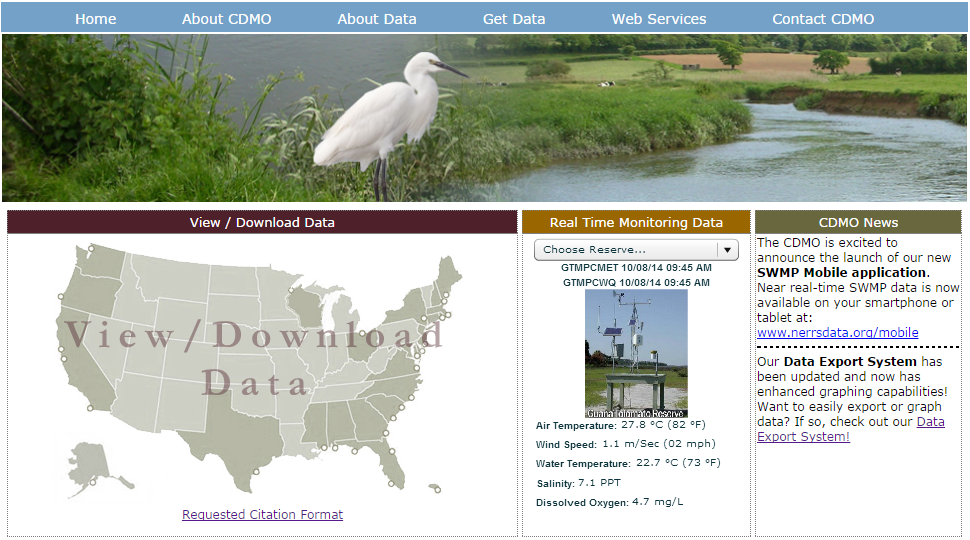
\includegraphics[width = \textwidth]{fig/cdmo_front.png}}
\end{frame}

%%%%%%
\begin{frame}{What is NERRS/SWMP?}
Hallmarks of SWMP - Standardized instruments and protocols, rigorous QAQC, very large dataset \\~\\
\begin{itemize}
\item All 28 reserves use identical instruments and standardized protocols \\~\\
\item All data are managed by the NERRS Centralized Data Management Office \\~\\
\item Database meets the definition of ``big data''
\end{itemize}
\end{frame}

%%%%%%
\begin{frame}[t]{What is NERRS/SWMP?}
As of April 30th, $>$ 63 million SWMP  data records available from CDMO\\~\\
Raw data will look like this...\\~\\
\centerline{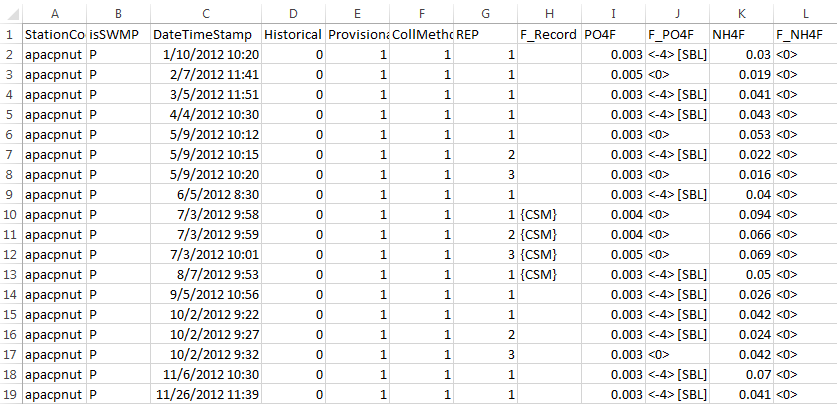
\includegraphics[width = 0.9\textwidth]{fig/qaqc_ex.png}}
\end{frame}

%%%%%%
\begin{frame}{What are the problems?}
An invaluable data source but no recent comparative analyses between systems \\~\\
NERRS researchers, managers, and technicians need more tools for trend analysis \\~\\
Some specific issues:\\~\\
\begin{itemize}
\item Knowing what data to use and how to obtain
\item Dealing with QAQC columns or removing `bad' observations
\item Combining data for comparison
\item Issues inherent with time series, e.g., signal vs. noise, data quantity
\end{itemize}
\end{frame}

%%%%%%
\begin{frame}{What are the needs?}
Several needs were identified given the challenges:\\~\\
\begin{itemize}
\item Understand regional and national trends while retaining the ability to determine local trends \\~\\
\item Train users \\~\\
\item Maintain a versatile and evolving data analysis approach \\~\\
\item Create a community of practice
\end{itemize}
\end{frame}

%%%%%%
\begin{frame}{
\includegraphics[width=0.05\paperwidth]{fig/muskrat.png}\hspace{0.07in}{\bf Genesis of SWMPrats}}
\centerline{\fbox{
\includegraphics[width = 0.95\textwidth]{fig/bg_main.jpg}}}
\vspace{0.2in}
One-day training workshop at 2014 annual meeting \\~\\
\begin{itemize}
\item Attended by over 70 NERRS staff, representing 19 of 28 reserves \\~\\
\item General focus on time series analysis, simple applications with SWMP data \\~\\
\item Pre/post workshop materials, including an R package for SWMP
\end{itemize}
\end{frame}

%%%%%%
\begin{frame}{
\includegraphics[width=0.05\paperwidth]{fig/muskrat.png}\hspace{0.07in}{\bf Genesis of SWMPrats}}
\centerline{\fbox{
\includegraphics[width = 0.95\textwidth]{fig/swmprats_logo.png}}}
\vspace{0.2in}
A working group was formed from this meeting \\~\\
\Large
\Bigtxt{S}ystem-\Bigtxt{W}ide \Bigtxt{M}onitoring \Bigtxt{P}rogram \Bigtxt{R}esources for the \Bigtxt{A}nalysis of \Bigtxt{T}ime \Bigtxt{S}eries \\~\\
\normalsize
\href{http://swmprats.net}{SWMPrats.net} is our base of operations...
\end{frame}

%%%%%%
\begin{frame}{
\includegraphics[width=0.05\paperwidth]{fig/muskrat.png}\hspace{0.07in}{\bf SWMPrats.net}}
\centerline{A website with information and tools for SWMP data analysis}
\vspace{0.1in}
\centerline{\fbox{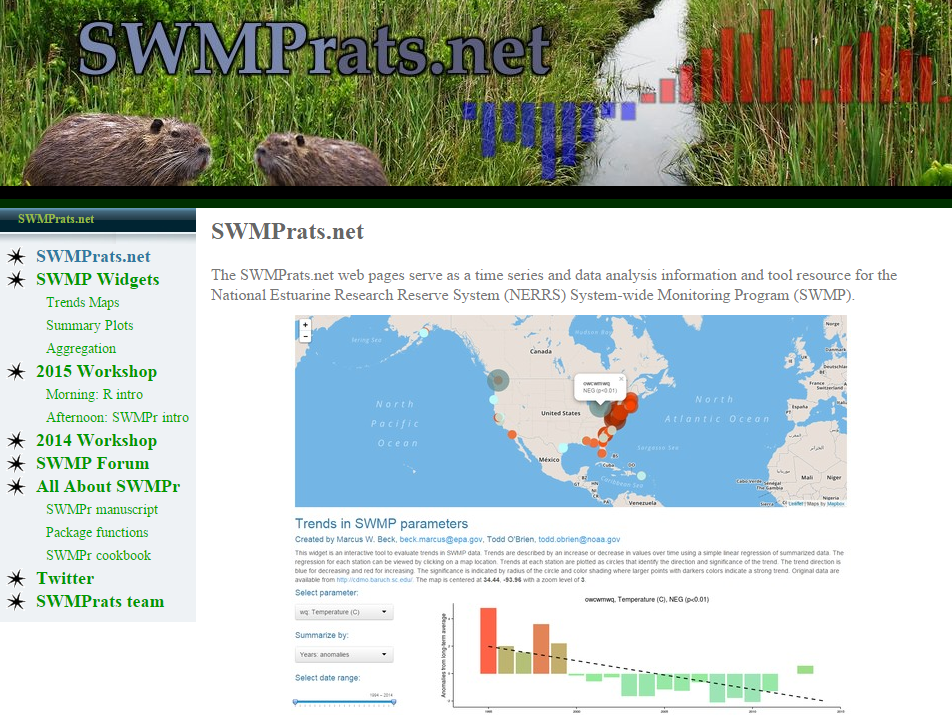
\includegraphics[width = 0.7\textwidth]{fig/swmprats_home.png}}}
\end{frame}

%%%%%%
\begin{frame}[fragile]{
\includegraphics[width=0.05\paperwidth]{fig/muskrat.png}\hspace{0.07in}{\bf SWMPrats.net: The SWMPr package}}
\centerline{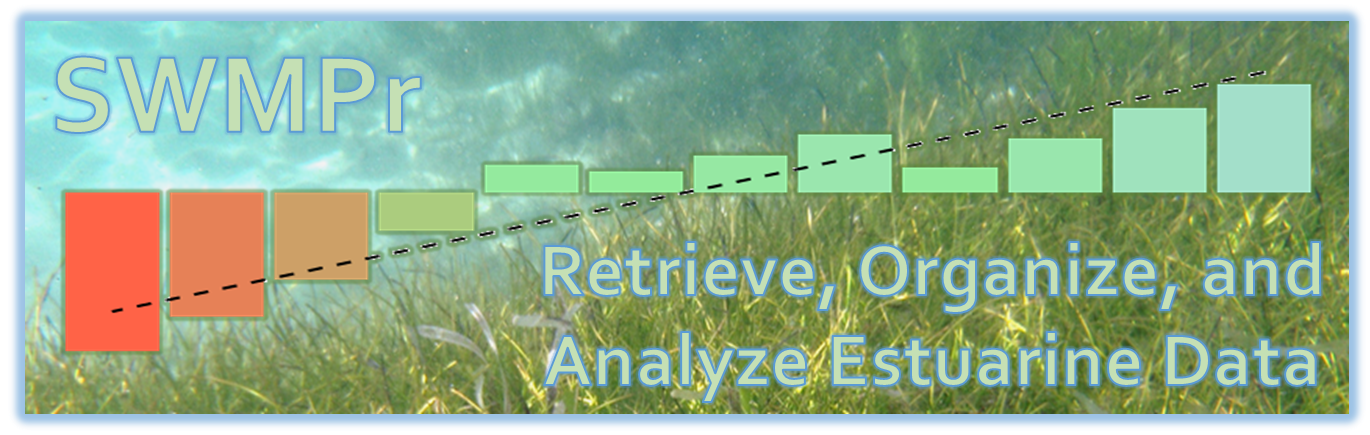
\includegraphics[width = 0.75\textwidth]{fig/swmpr_logo.png}}
\vspace{0.15in}
SWMPr is an open-source R package described on the website, v2.1.5 is \href{http://cran.r-project.org/web/packages/SWMPr/index.html}{now available}
\begin{knitrout}
\definecolor{shadecolor}{rgb}{0.941, 0.976, 0.91}\color{fgcolor}\begin{kframe}
\begin{alltt}
\hlstd{> }\hlcom{# install/load from R}
\hlstd{> }\hlkwd{install.packages}\hlstd{(}\hlstr{'SWMPr'}\hlstd{)}
\hlstd{> }\hlkwd{library}\hlstd{(SWMPR)}
\end{alltt}
\end{kframe}
\end{knitrout}
\end{frame}

%%%%%%
\begin{frame}[fragile]{
\includegraphics[width=0.05\paperwidth]{fig/muskrat.png}\hspace{0.07in}{\bf SWMPrats.net: The SWMPr package}}
The software addresses the unglamorous but necessary challenges of analyzing time series, specific to SWMP \\~\\
What are some challenges? \\~\\
\begin{columns}
\begin{column}{0.6\textwidth}
\begin{itemize}
\item Dealing with `bad' data \\~\\
\item Subsetting by date ranges, parameters \\~\\
\item Combining data from different sites \\~\\
\item Standardizing time steps \\~\\
\item ...and analysis
\end{itemize}
\end{column}
\begin{column}{0.4\textwidth}
\centerline{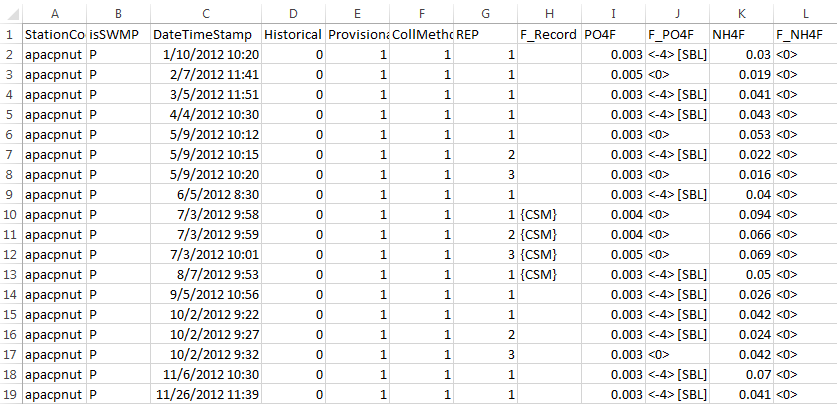
\includegraphics[width = 0.9\textwidth]{fig/qaqc_ex.png}}
\end{column}
\end{columns}
\end{frame}

%%%%%%
\begin{frame}[fragile]{
\includegraphics[width=0.05\paperwidth]{fig/muskrat.png}\hspace{0.07in}{\bf SWMPrats.net: The SWMPr package}}
Package description published in The R Journal this year \\~\\ 
\centerline{\fbox{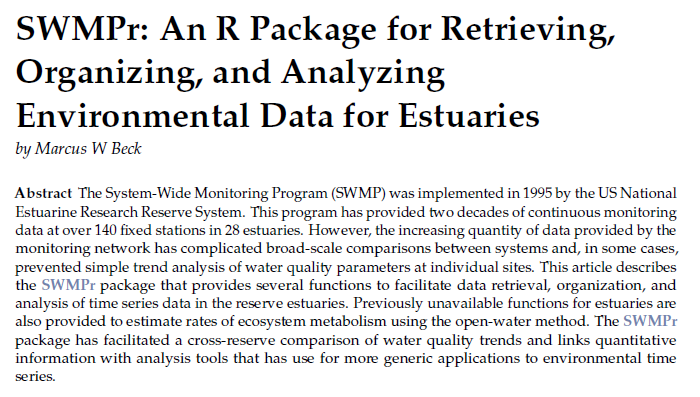
\includegraphics[width=0.85\textwidth]{fig/SWMPr_manu.png}}}
\end{frame}

%%%%%%
\begin{frame}[t]{What can SWMPr do?}
SWMPr functions are grouped into three categories that describe their use in the `data workflow' \\~\\
\begin{columns}[t]
\begin{column}{0.3\textwidth}
\Bigtxt{Retrieve}\\~\\
\small{
\texttt{all\_params}\\
\texttt{all\_params_dtrng}\\
\texttt{import\_local}\\
\texttt{import\_remote}\\
\texttt{single\_param}\\
\texttt{site\_codes}\\
\texttt{site\_codes\_ind}
}
\end{column}
\begin{column}{0.3\textwidth}
\Bigtxt{Organize}\\~\\
\small{
\texttt{comb}\\
\texttt{qaqc}\\
\texttt{qaqcchk}\\
\texttt{rem\_reps}\\
\texttt{setstep}\\
\texttt{subset}\\
}
\end{column}
\begin{column}{0.3\textwidth}
\Bigtxt{Analyze}\\~\\
\small{
\texttt{aggreswmp}\\
\texttt{aggremetab}\\
\texttt{ecometab}\\
\texttt{decomp}\\
\texttt{decomp\_cj}\\
\texttt{hist}\\
\texttt{lines}\\
\texttt{na.approx}\\
\texttt{plot}\\
\texttt{plot\_metab}\\
\texttt{plot\_summary}\\
\texttt{smoother}\\
}
\end{column}
\end{columns}
\end{frame}

%%%%%%
\begin{frame}[fragile]{
\includegraphics[width=0.05\paperwidth]{fig/muskrat.png}\hspace{0.07in}{\bf SWMPrats.net: The SWMPr package}}
Proof of concept, import and combine wq and weather data from Apalachicola Bay
\begin{knitrout}
\definecolor{shadecolor}{rgb}{0.941, 0.976, 0.91}\color{fgcolor}\begin{kframe}
\begin{alltt}
\hlstd{> }\hlcom{# import data}
\hlstd{> }\hlkwd{data}\hlstd{(apaebmet)}
\hlstd{> }\hlkwd{data}\hlstd{(apacpwq)}
\hlstd{> }\hlstd{met} \hlkwb{<-} \hlstd{apaebmet}
\hlstd{> }\hlstd{wq} \hlkwb{<-} \hlstd{apacpwq}
\hlstd{> }
\hlstd{> }\hlcom{# combine, two hours time step}
\hlstd{> }\hlcom{# only overlapping date ranges}
\hlstd{> }\hlstd{dat} \hlkwb{<-} \hlkwd{comb}\hlstd{(met, wq,} \hlkwc{timestep} \hlstd{=} \hlnum{120}\hlstd{,}
\hlstd{+ }  \hlkwc{method} \hlstd{=} \hlstr{'intersect'}\hlstd{)}
\end{alltt}
\end{kframe}
\end{knitrout}
Try doing the same by hand...
\end{frame}

%%%%%
\begin{frame}[fragile]{
\includegraphics[width=0.05\paperwidth]{fig/muskrat.png}\hspace{0.07in}{\bf SWMPrats.net: The SWMPr package}}
Example: fill missing data with \texttt{na.approx} \\~\\
\begin{knitrout}\scriptsize
\definecolor{shadecolor}{rgb}{0.941, 0.976, 0.91}\color{fgcolor}

{\centering 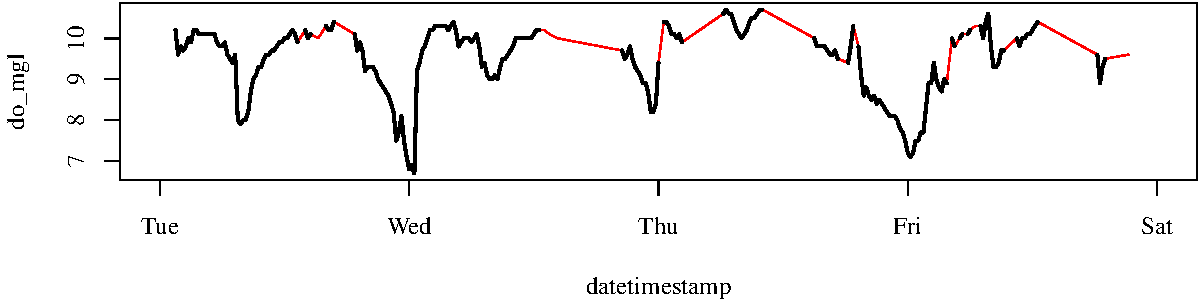
\includegraphics[width=0.85\textwidth]{fig//filled-1} 

}



\end{knitrout}
Example: smooth data with \texttt{smoother} \\~\\
\begin{knitrout}\scriptsize
\definecolor{shadecolor}{rgb}{0.941, 0.976, 0.91}\color{fgcolor}

{\centering 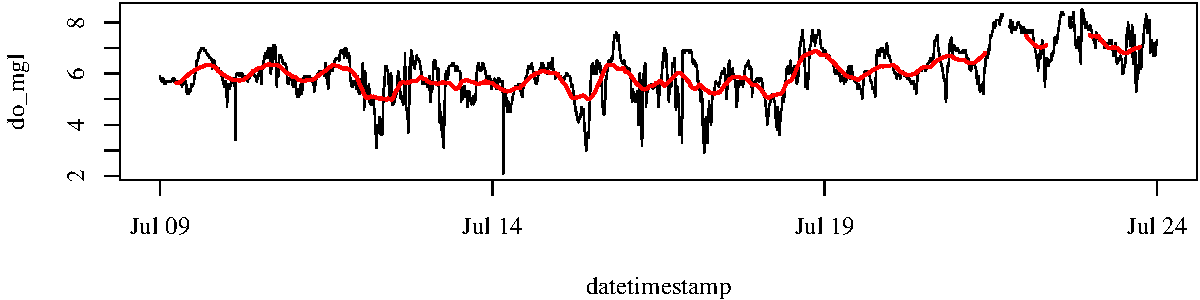
\includegraphics[width=0.85\textwidth]{fig//smooth-1} 

}



\end{knitrout}
\end{frame}

%%%%%%
\begin{frame}[fragile]{
\includegraphics[width=0.05\paperwidth]{fig/muskrat.png}\hspace{0.07in}{\bf SWMPrats.net: The SWMPr package}}
Example: time series decomposition with \texttt{decomp\_cj} (chl-a at cbmocnut)\\~\\
\begin{knitrout}
\definecolor{shadecolor}{rgb}{0.941, 0.976, 0.91}\color{fgcolor}

{\centering 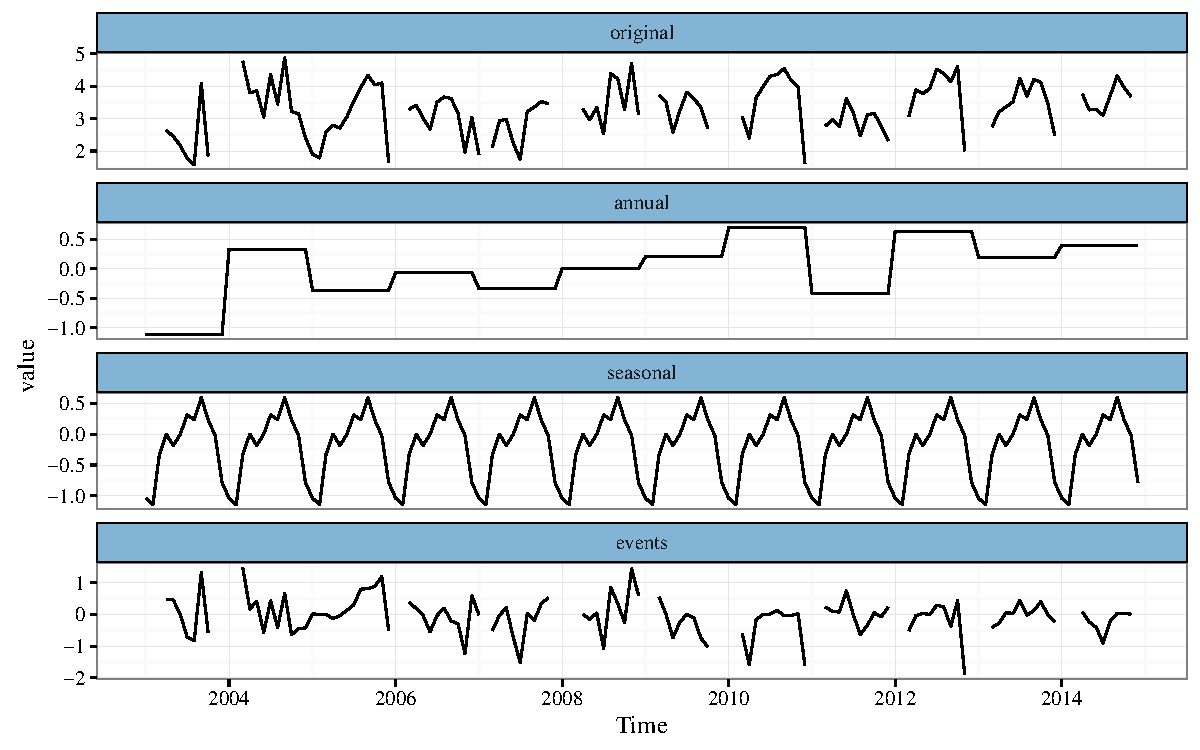
\includegraphics[width=0.85\textwidth]{fig/decomp_dep-1} 

}



\end{knitrout}
\end{frame}

%%%%%%
\begin{frame}[fragile]{
\includegraphics[width=0.05\paperwidth]{fig/muskrat.png}\hspace{0.07in}{\bf SWMPrats.net: The SWMPr package}}
Example: estimate ecosystem metabolism with \texttt{ecometab} (apadbwq)

\begin{knitrout}
\definecolor{shadecolor}{rgb}{0.941, 0.976, 0.91}\color{fgcolor}

{\centering 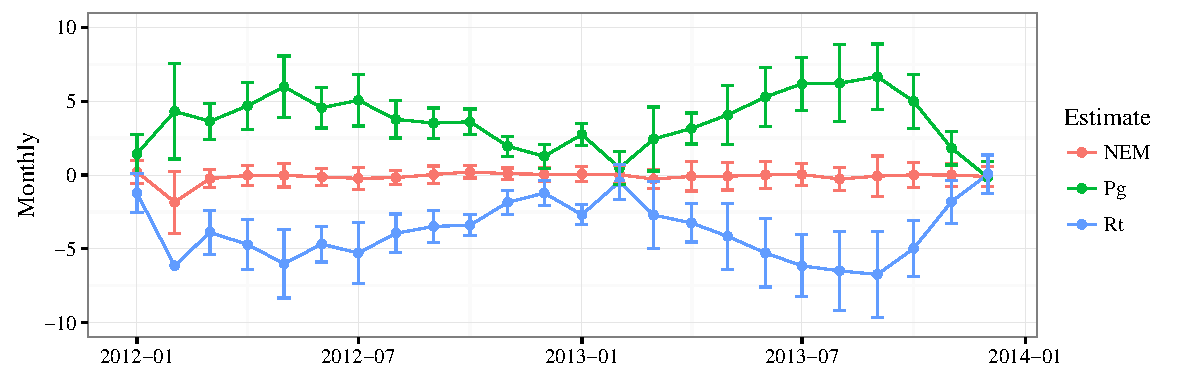
\includegraphics[width=0.95\textwidth]{fig//ecometab1-1} 

}



\end{knitrout}
\begin{knitrout}
\definecolor{shadecolor}{rgb}{0.941, 0.976, 0.91}\color{fgcolor}

{\centering 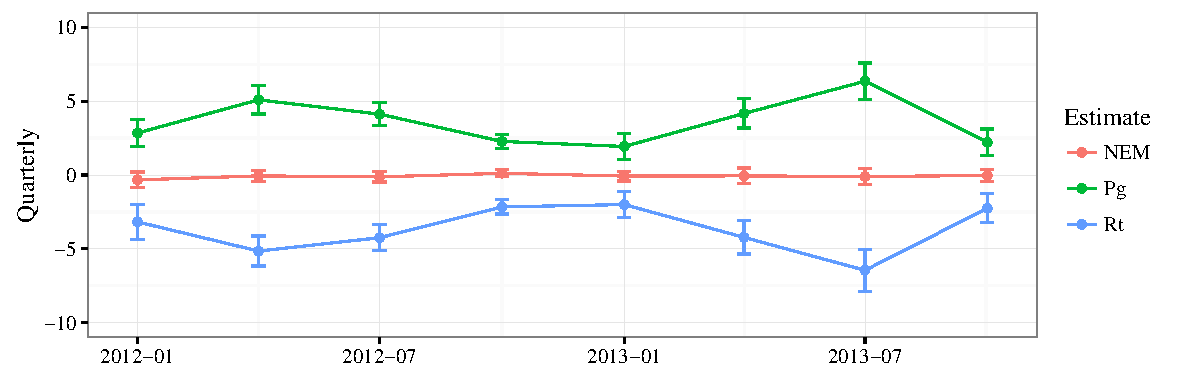
\includegraphics[width=0.95\textwidth]{fig//ecometab2-1} 

}



\end{knitrout}
\end{frame}

%%%%%%
\begin{frame}[fragile]{
\includegraphics[width=0.05\paperwidth]{fig/muskrat.png}\hspace{0.07in}{\bf SWMPrats.net: Widgets}}
The most common question - has there been a change over time at my site? \\~\\
The functions in the package can help answer this very general question...\\~\\
...but it's often easier to interactively evaluate the data! \\~\\
Two shiny applications, hosted on \href{http://www.shinyapps.io/}{shinyapps.io}, allow users to visualize trends in SWMP data \\~\\
These apps were created with SWMPr functions or use them `reactively'
\end{frame}

%%%%%%
\begin{frame}[t, fragile]{
\includegraphics[width=0.05\paperwidth]{fig/muskrat.png}\hspace{0.07in}{\bf SWMPrats.net: Widgets}}
SWMP summary plots: \href{https://beckmw.shinyapps.io/swmp_summary/}{https://beckmw.shinyapps.io/swmp\_summary/}\\~\\
\centerline{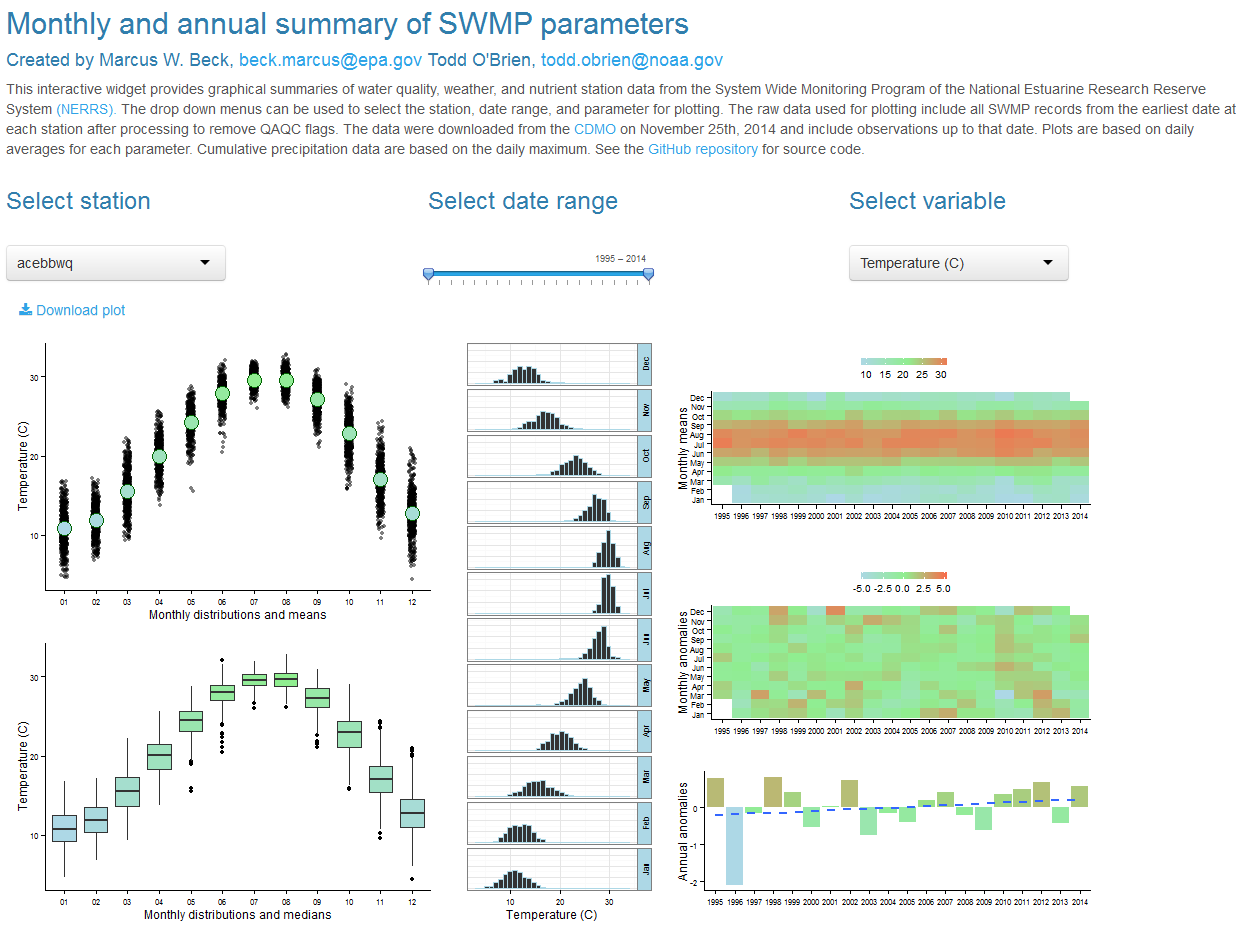
\includegraphics[width = 0.62\textwidth]{fig/swmp_summary.png}}
\end{frame}

%%%%%%
\begin{frame}[t, fragile]{
\includegraphics[width=0.05\paperwidth]{fig/muskrat.png}\hspace{0.07in}{\bf SWMPrats.net: Widgets}}
SWMP trends map: \href{https://beckmw.shinyapps.io/swmp_comp/}{https://beckmw.shinyapps.io/swmp\_comp/}\\~\\
\centerline{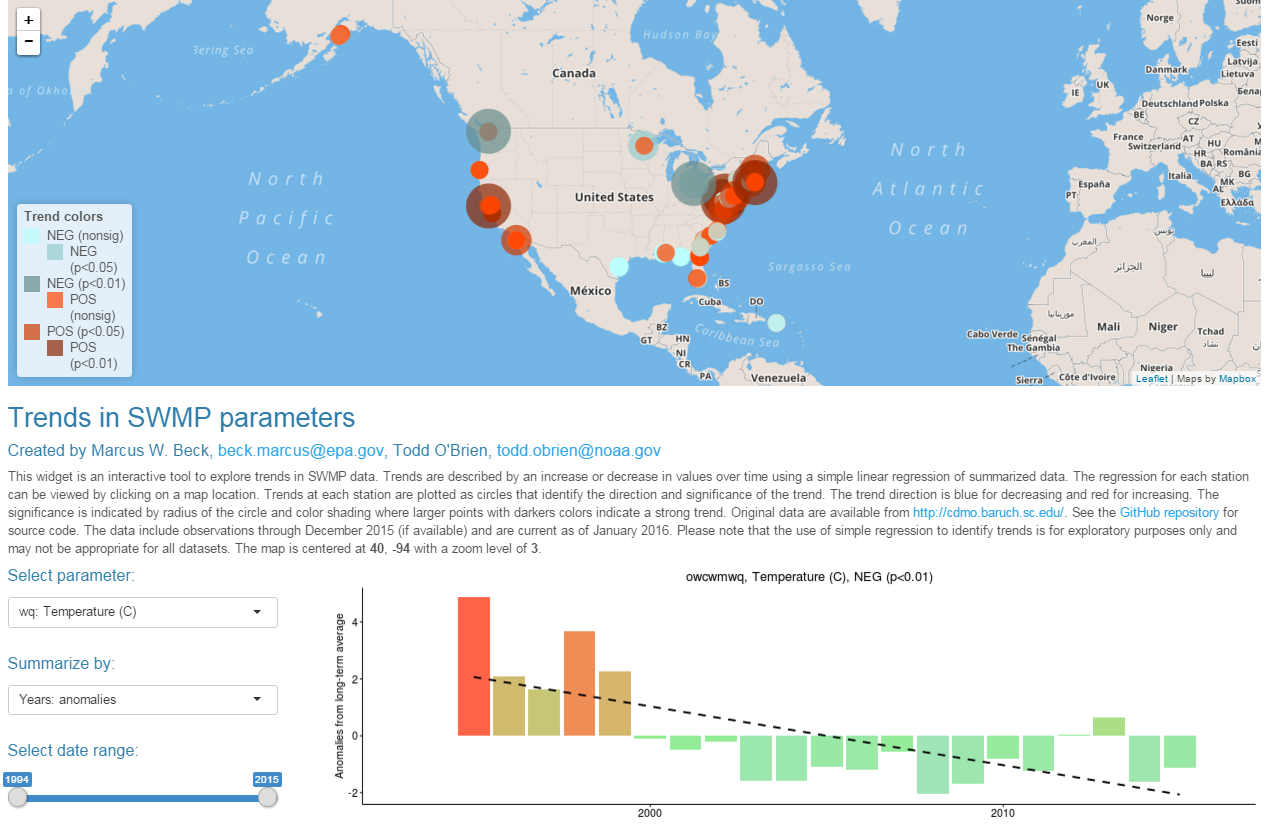
\includegraphics[width = 0.82\textwidth]{fig/swmp_comp.png}}
\end{frame}

%%%%%%
\begin{frame}[t, fragile]{
\includegraphics[width=0.05\paperwidth]{fig/muskrat.png}\hspace{0.07in}{\bf SWMPrats.net: Widgets}}
SWMP aggregation: \href{https://beckmw.shinyapps.io/swmp_agg/}{https://beckmw.shinyapps.io/swmp\_agg/}\\~\\
\centerline{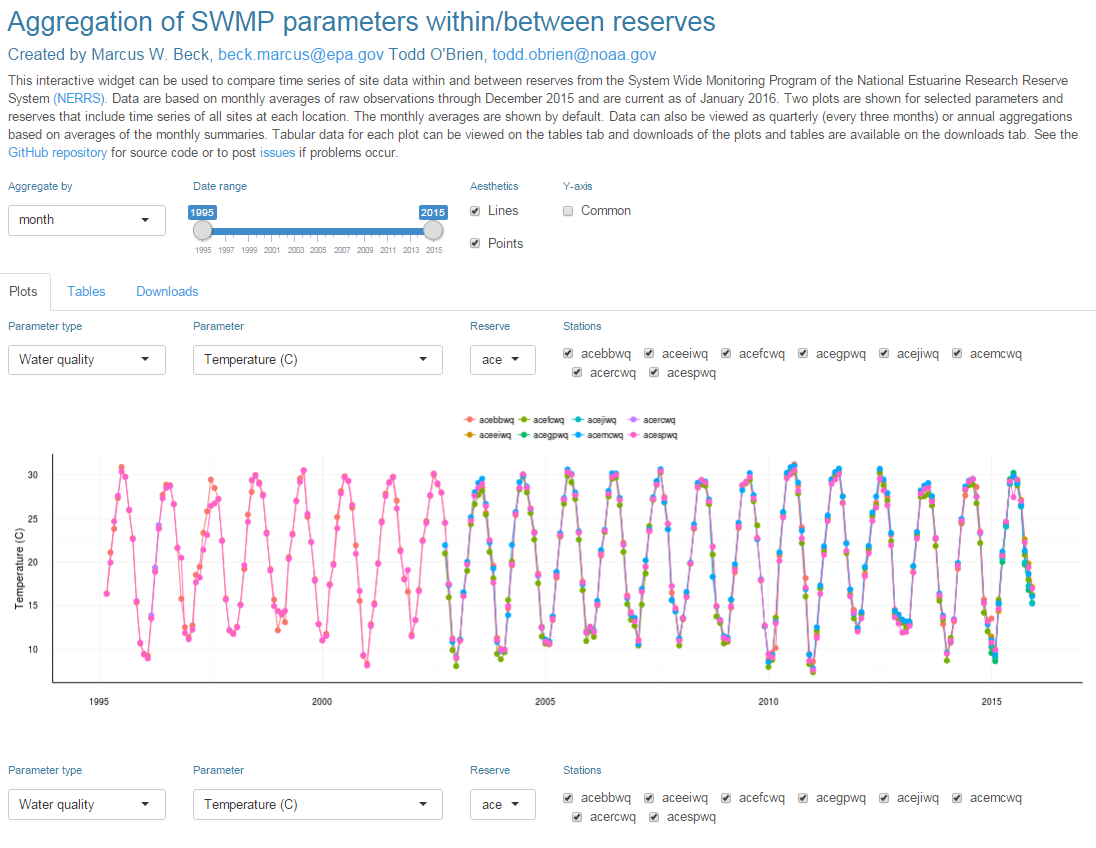
\includegraphics[width = 0.7\textwidth]{fig/swmp_agg.png}}
\end{frame}

%%%%%%
\begin{frame}[t, fragile]{
\includegraphics[width=0.05\paperwidth]{fig/muskrat.png}\hspace{0.07in}{\bf SWMPrats.net: Forum}}
\centerline{Last but not least, a discussion \href{http://swmprats.net/forum}{forum} for all things analytical}
\vspace{0.1in}
\centerline{\fbox{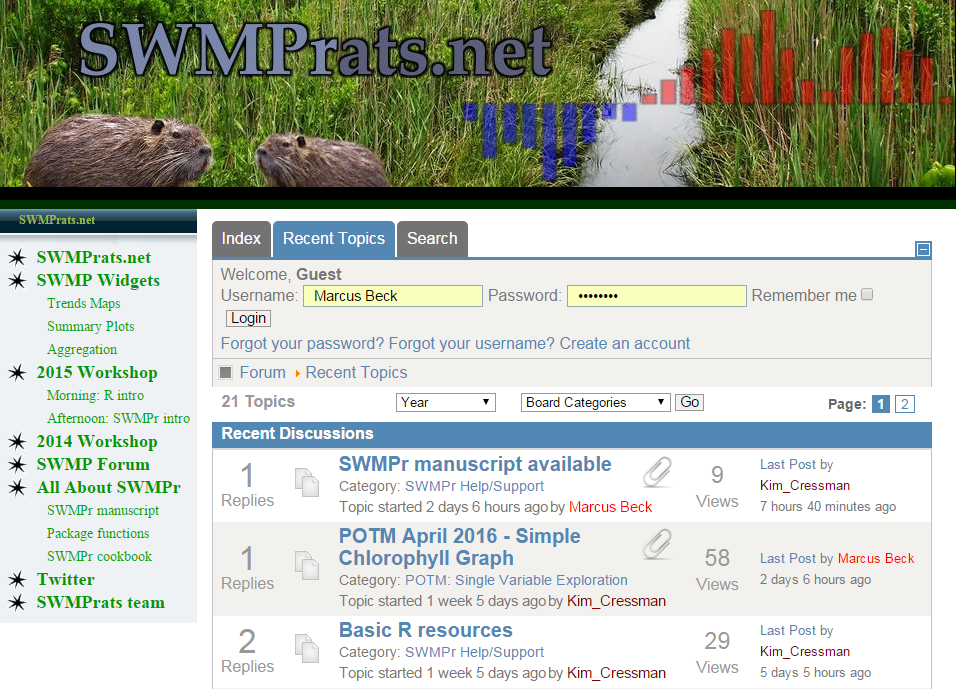
\includegraphics[width = 0.75\textwidth]{fig/swmprats_forum.png}}}
\end{frame}

%%%%%%
\begin{frame}[t, fragile]{
\includegraphics[width=0.05\paperwidth]{fig/muskrat.png}\hspace{0.07in}{\bf SWMPrats.net: Forum}}
\centerline{Last but not least, a discussion \href{http://swmprats.net/forum}{forum} for all things analytical}
\vspace{0.1in}
\centerline{\fbox{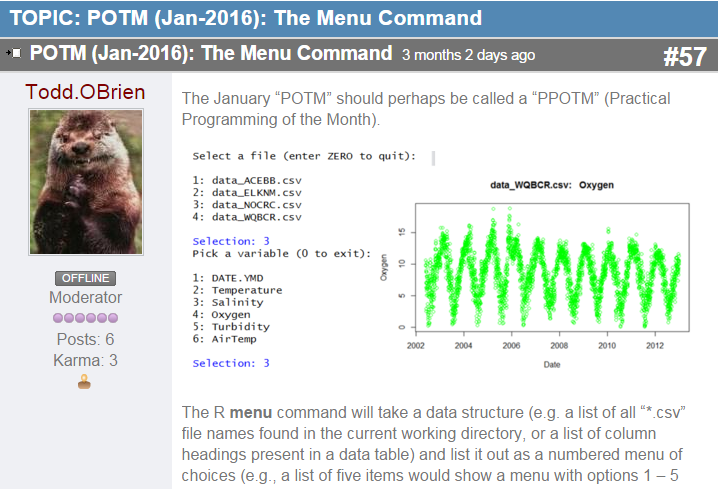
\includegraphics[width = 0.75\textwidth]{fig/POTM.png}}}
\end{frame}

%%%%%%
\begin{frame}[fragile]{
\includegraphics[width=0.05\paperwidth]{fig/muskrat.png}\hspace{0.07in}{\bf Continuing work and engagement}}
SWMPrats.net is in its infancy but already seeing heavy use \\~\\
\begin{itemize}
\item 3140 downloads of SWMPr to date
\item Apps have been used 160 hours in the last three months \\~\\
\end{itemize}
Additional training workshops Oct. 2015, planned for 2016 \\~\\
\begin{columns}
\begin{column}{0.45\textwidth}
\centerline{\fbox{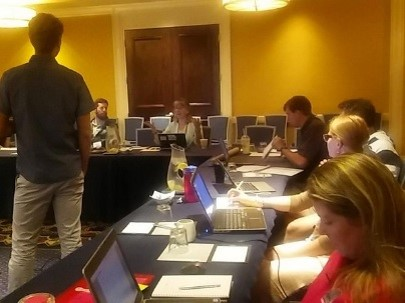
\includegraphics[width = 0.85\textwidth]{fig/work1.jpg}}}
\end{column}
\begin{column}{0.45\textwidth}
\centerline{\fbox{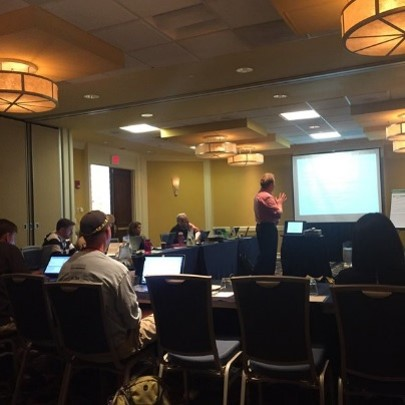
\includegraphics[width = 0.64\textwidth]{fig/work2.jpg}}}
\end{column}
\end{columns}
\end{frame}

%%%%%%
\begin{frame}[t, fragile]{
\includegraphics[width=0.05\paperwidth]{fig/muskrat.png}\hspace{0.07in}{\bf Continuing work and engagement}}
\begin{columns}
\begin{column}{0.53\textwidth}
\centerline{\fbox{
\includegraphics[width = \textwidth]{fig/swmprats_logo.png}}}
\end{column}
\begin{column}{0.43 \textwidth}
\centerline{\fbox{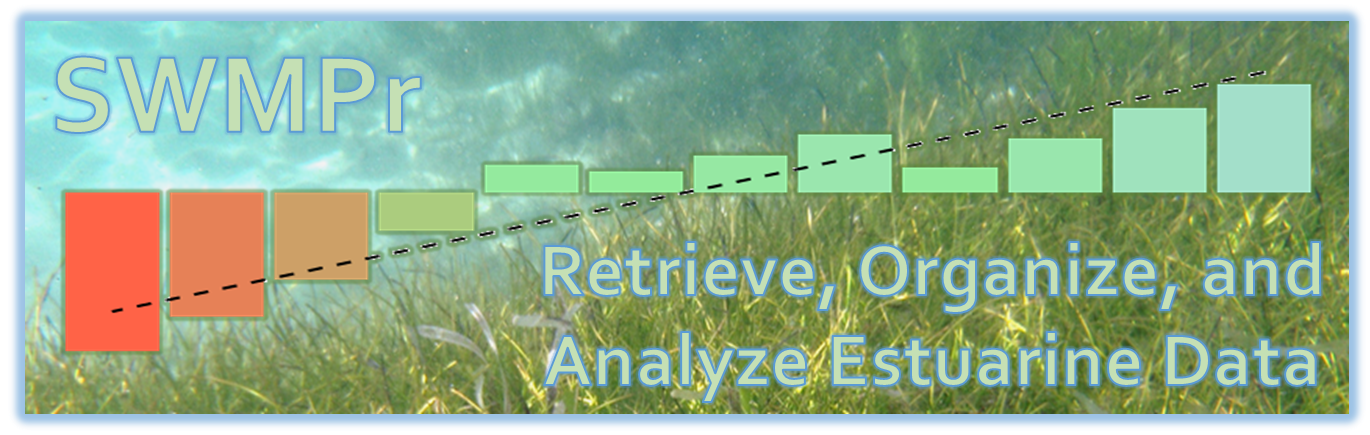
\includegraphics[width = 0.78\textwidth]{fig/swmpr_logo.png}}}
\end{column}
\end{columns}
\vspace{0.2in}
SWMPrats is an ad hoc group formed organically from the NERRS community \\~\\
Success depends on:\\~\\
\begin{itemize}
\item Healthy discourse between the creators and users \\~\\
\item In-person training workshops\\~\\
\item Benefits of open-source resources
\end{itemize}
\end{frame}

%%%%%%
\begin{frame}[t, fragile]{
\includegraphics[width=0.05\paperwidth]{fig/muskrat.png}\hspace{0.07in}{\bf Continuing work and engagement}}
\begin{columns}
\begin{column}{0.53\textwidth}
\centerline{\fbox{
\includegraphics[width = \textwidth]{fig/swmprats_logo.png}}}
\end{column}
\begin{column}{0.43 \textwidth}
\centerline{\fbox{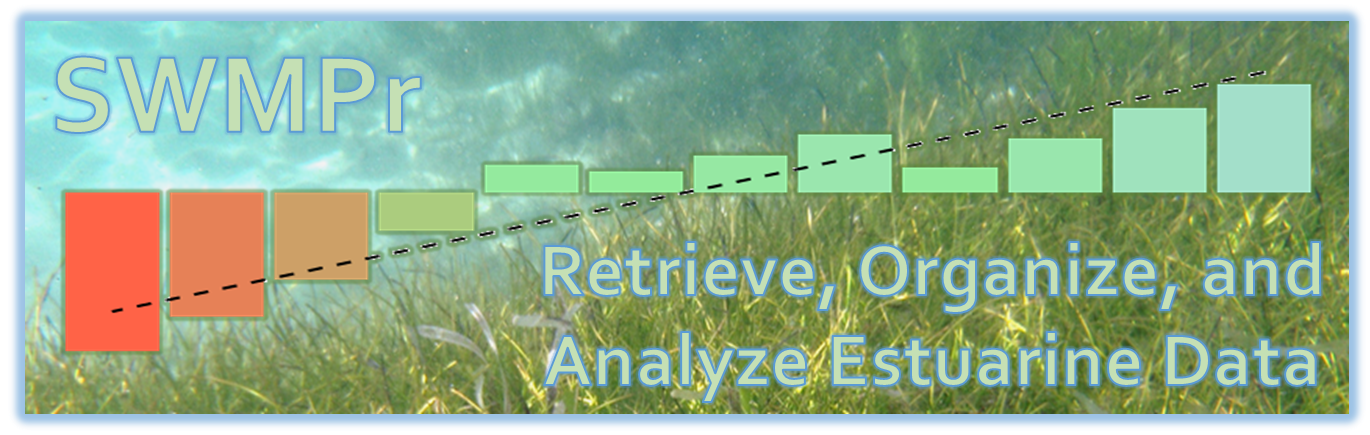
\includegraphics[width = 0.78\textwidth]{fig/swmpr_logo.png}}}
\end{column}
\end{columns}
\vspace{0.2in}
\begin{itemize}
\item SWMP data are now more accessible and analyses are tractable\\~\\
\item Site, regional, and national comparisons provide capacity to develop understanding of climate and anthropogenic drivers of change in estuarine systems \\~\\
\item As the dataset expands, these tools will facilitate evaluation of long-term trends within and between locations
\end{itemize}
\end{frame}

%%%%%%
\begin{frame}[t, fragile]{
\includegraphics[width=0.05\paperwidth]{fig/muskrat.png}\hspace{0.07in}{\bf Continuing work and engagement}}
\begin{columns}
\begin{column}{0.53\textwidth}
\centerline{\fbox{
\includegraphics[width = \textwidth]{fig/swmprats_logo.png}}}
\end{column}
\begin{column}{0.43 \textwidth}
\centerline{\fbox{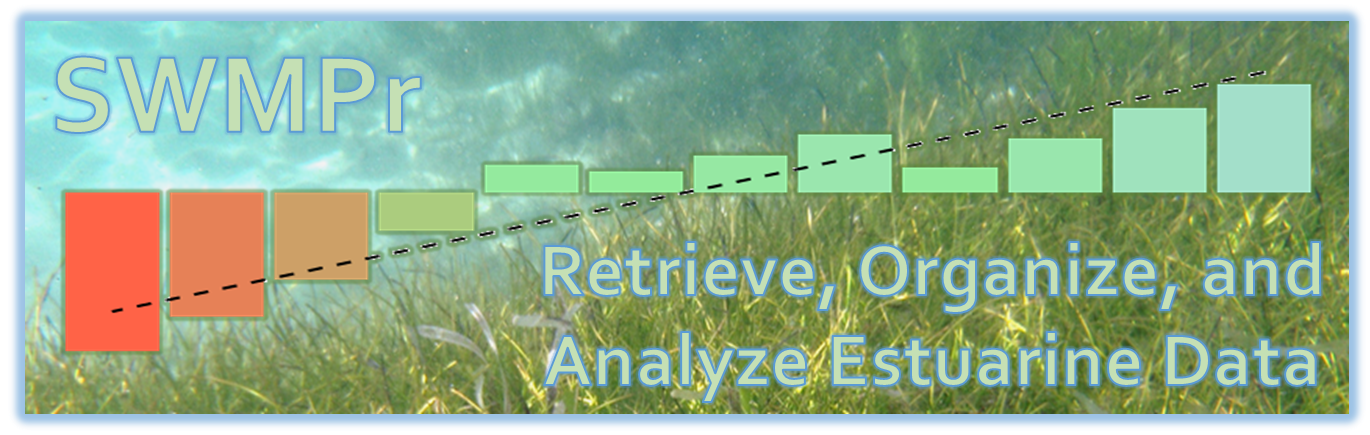
\includegraphics[width = 0.78\textwidth]{fig/swmpr_logo.png}}}
\end{column}
\end{columns}
\vspace{0.2in}
Contacts: \includegraphics[width=0.05\paperwidth]{fig/muskrat2.png}\hspace{0.05in}\href{mailto:beck.marcus@epa.gov}{beck.marcus@epa.gov}, \includegraphics[width=0.05\paperwidth]{fig/muskrat2.png}\hspace{0.05in}\href{mailto:todd.obrien@noaa.gov}{todd.obrien@noaa.gov}, \includegraphics[width=0.05\paperwidth]{fig/muskrat2.png}\hspace{0.05in}\href{mailto:marie.bundy@noaa.gov}{marie.bundy@noaa.gov}  \\~\\
To get this presentation: \href{https://github.com/fawda123/NWQMC_16}{https://github.com/fawda123/NWQMC\_16} \\~\\
Apps: \href{http://swmprats.net/swmp-widgets/summary-plots}{http://swmprats.net/swmp-widgets/summary-plots}, \href{http://swmprats.net/swmp-widgets/trends-maps}{http://swmprats.net/swmp-widgets/trends-maps}, \href{http://swmprats.net/swmp-widgets/swmp-widget-aggregation}{http://swmprats.net/swmp-widgets/swmp-widget-aggregation} \\~\\
Visit the development site for the most recent version of SWMPr: \href{https://github.com/fawda123/SWMPr}{https://github.com/fawda123/SWMPr}\\~\\
\end{frame}

\end{document}
